\documentclass[12pt]{scrartcl}
 
\usepackage[margin=1in]{geometry} 
\usepackage{amsmath,amsthm,amssymb}
\usepackage{hyperref}
\usepackage{listings}			% Für Quellcode
\usepackage{graphicx}
\usepackage{tabularx}			% für Tabellen mit gleicher Spaltenbreite und automatischen
\usepackage{fontspec}
\defaultfontfeatures{Mapping=tex-text}
\setsansfont{Source Sans Pro}
\setmainfont{Source Sans Pro}
\usepackage[babel, german=quotes]{csquotes} % einfache Handhabung von quotations
\usepackage[backend=biber]{biblatex} %biblatex mit biber laden
\ExecuteBibliographyOptions{
sorting=nyt, %Sortierung Autor, Titel, Jahr
bibwarn=true, %Probleme mit den Daten, die Backend betreffen anzeigen
isbn=false, %keine isbn anzeigen
url=false %keine url anzeigen
}
\addbibresource{lit.bib} %Bibliographiedateien laden

\begin{document}
 
% --------------------------------------------------------------
%                         Start here
% --------------------------------------------------------------
 
%\renewcommand{\qedsymbol}{\filledbox}
 
\title{Final Course Assignment \\ }%replace X with the appropriate number
\author{Mark Niehues, Stefaan Hessmann \\ %replace with your name
Mathematical Aspects in Machine Learning} %if necessary, replace with your course title

\maketitle
 
\section{Introduction}
In the past course we dealt with the broad mathematical foundations of machine learning. To get an idea of what the consequences of those mathematical theorems and approaches are and to get in touch with the standard Python tools, we have evaluated an comparatively easy data science example found on \url{kaggle.com}. The example dataset \cite{Kaggle2017} consists of the historic passenger records of the disastrous Titanic maiden voyage in 1912. 

\begin{figure}
  \centering
    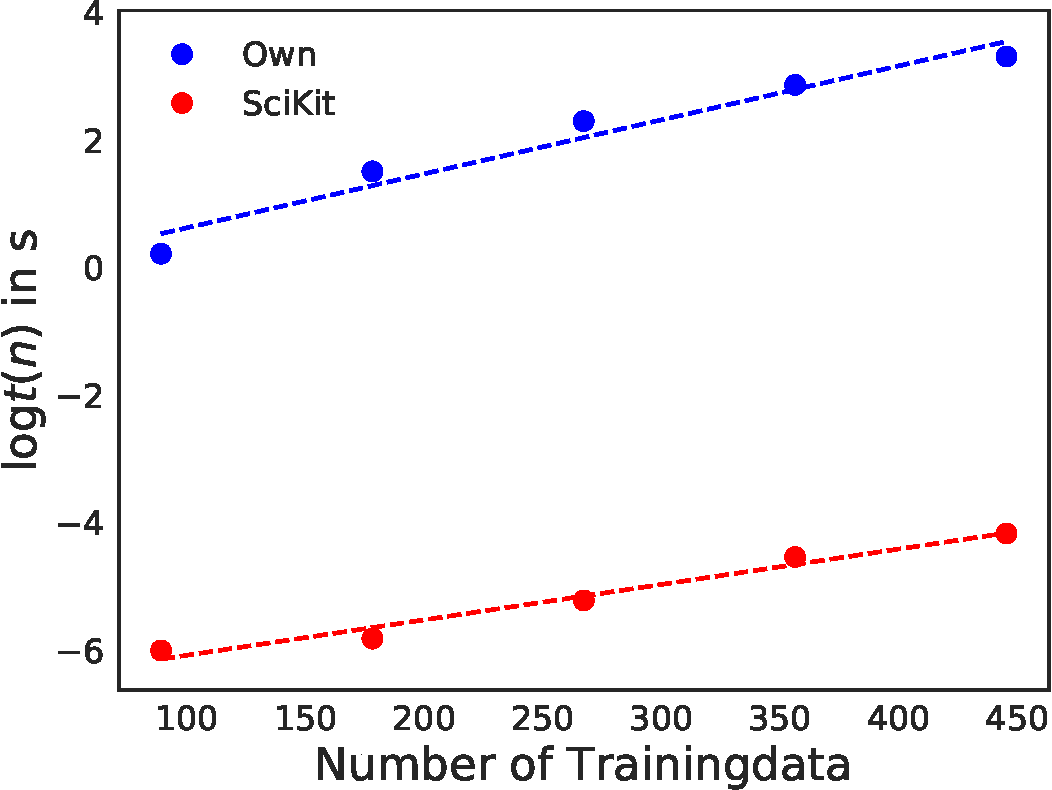
\includegraphics[width=0.5\textwidth]{media_saved/benchmark}
  \caption{Benchmark}
  \label{fig:gull}
\end{figure}

\lstinputlisting[language=Python,									% Style
	caption={Hello World},		% Beschriftung
	firstnumber={0},										% Start der Nummerierung
	firstline={0}											% 1. Codezeile
]											% letzte Codezeile
{./own_svm/kernels.py}


\section{Applying Machine Learning Methods on the Titanic Disaster}
blalba
\section{Implementation of an easy SMO Algorithm}

\printbibliography %hier Bibliographie ausgeben lassen
\end{document}        